\documentclass{jarticle}

\usepackage[dvipdfmx]{graphicx}
\usepackage{float}
\usepackage{url}

\title{光速度の測定}
\author{2511198 肥田幸久 \\ 共同実験者 \\ 2511238 矢吹千陽}
\date{2025年5月22日}

\begin{document}
\maketitle



\section{実験の目的}
光速度は物理学のもっとも基本的な定数のひとつであり, 国際単位系の$\mathrm{m}$の定義にも採用されている. 本実験ではこの光速度と, それに加えて同軸ケーブルを伝わる信号の速度の測定を行う.



\section{実験の原理}


\subsection{光速度の測定}

光速度の測定には, 木星の衛星の食, 光行差, 回転歯車, 回転鏡など歴史的にさまざまな方法が用いられてきた. 本実験では, それらに比べてシンプルかつ直接的な方法である「距離と時間の差」により、光速度を測定する.

光速度$c$は, 距離$d$を光が移動するのにかかる時間$t$を用いて,
\begin{equation}
  c=\frac{d}{t}
\end{equation}
と表される. この関係は本実験のもっとも根本的な原理である.

本実験では, 同一のパルスレーザー光を短距離経路と長距離経路に分岐させ, それぞれの往復にかかる時間を比較する. 両者の時間差$T$と光路差$L$を用いて光速度$c$は以下のように表される.
\begin{equation}
  c=\frac{L}{T}
\end{equation}
これにより, 絶対的な時間や距離を測定することなく, 高精度な光速度の測定が可能となる.


\subsection{同軸ケーブルを伝わる信号速度の測定}

パルス発生器から半導体レーザーに接続されている同軸ケーブルをインピーダンス整合器ごと取り外すと, インピーダンスの整合がとれないため終端で信号パルスが反射する.

この実験では, パルス発生器から直接観測したパルスと終端の反射によって生じたパルスとの時間間隔$T$を測定する.
このパルスの時間間隔$T$と同軸ケーブルの長さを$L$を用いて, 同軸ケーブルを伝わる信号速度$v$は以下のように表される.
\begin{equation}
  v=\frac{2L}{T}
\end{equation}



\section{実験方法}


\subsection{光速度の測定}

本実験では以下のような装置を用いて測定を行った.
図中の半導体レーザー(レーザーダイオード)は波長$685\,\mathrm{nm}$の赤色光を出す.
そこでパルス発生器からレーザーに電圧を加え, 幅約$10\,\mathrm{ns}$の光パルスを出力させる.
この短い光パルスを観測するために, 応答時間が$1\,\mathrm{nm}$以下の光検出器, ここではpinフォトダイオード(pin接合のダイオード)を使用する.

\begin{figure}[H]
  \begin{center}
    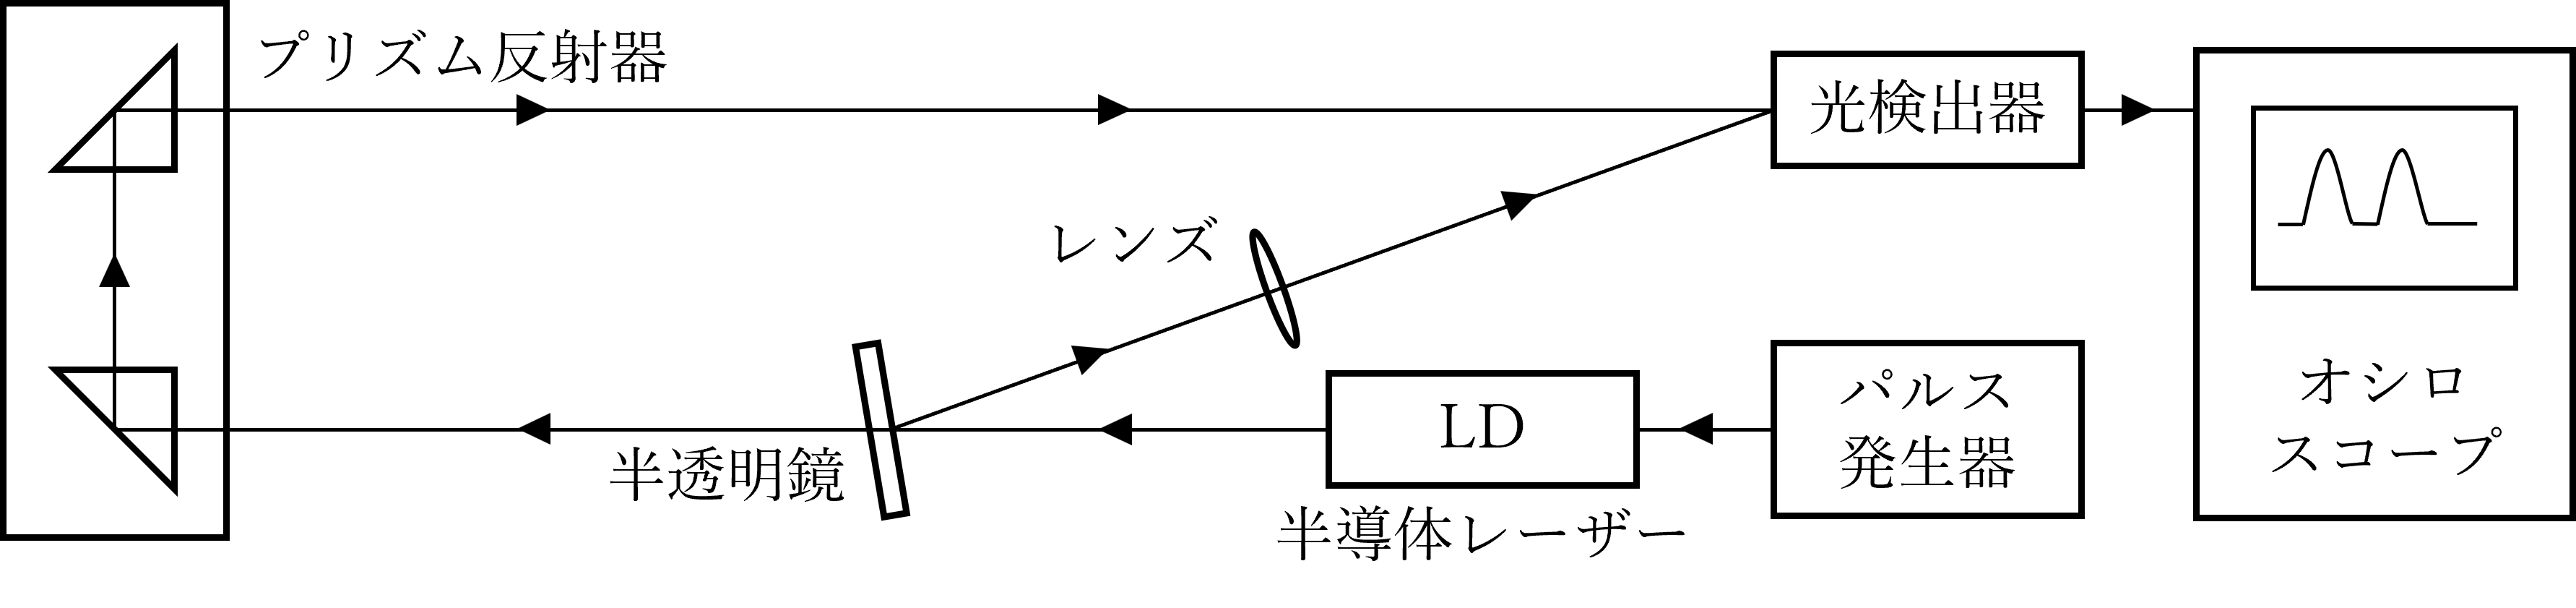
\includegraphics[width=110mm]{experimental_method_picture.png}
    \caption{光速度の測定装置}
  \end{center}
\end{figure}

測定では, 半導体レーザーから繰り返し周波数約$15\,\mathrm{MHz}$の光パルスを数$\mathrm{m}$離れたプリズム反射器で反射させて光検出器に導く.
また, 半導体レーザーとプリズム反射器の間でレーザーの一部を半透明鏡で反射させ, 同じ光検出器に導く.

光検出器の出力信号をオシロスコープに導き, 2つの光パルスの時間間隔$T$を測定する.
加えて, プリズム反射器を通じて光検出器に入る光路(長距離経路)と, 半透明鏡を通じて光検出器に入る光路(短距離経路)との差$L$を測定する.

\begin{figure}[H]
  \begin{center}
    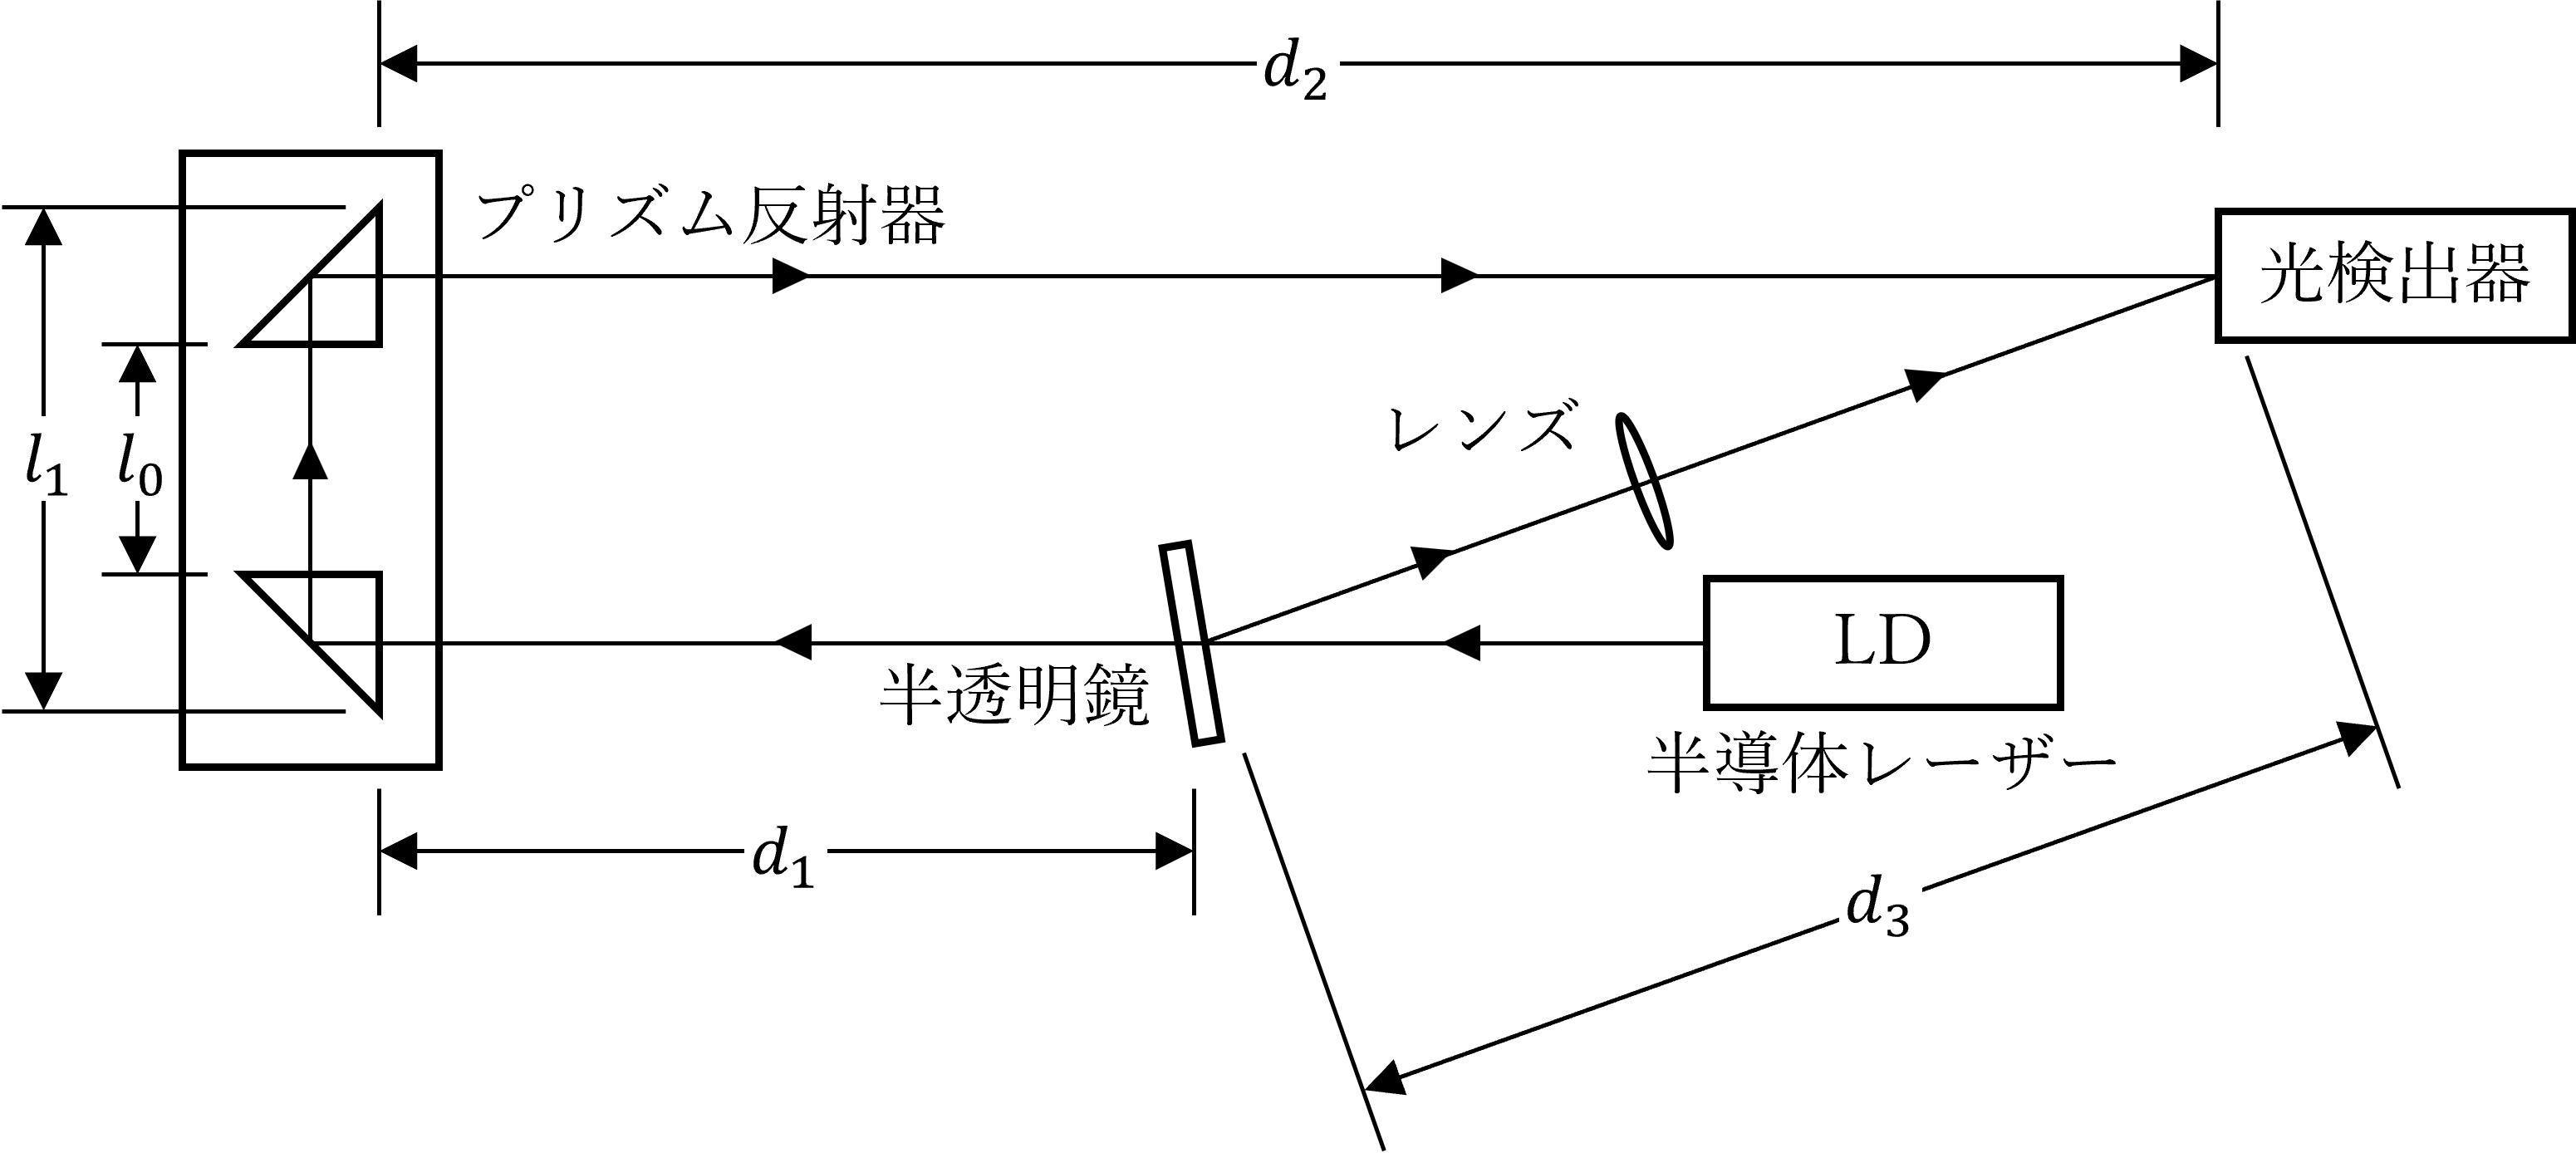
\includegraphics[width=95mm]{experimental_distance_picture.png}
    \caption{光路の測定}
  \end{center}
\end{figure}

プリズムのガラスの屈折率を$n$とすると, 光路差$L$は以下の式で求められる.
\begin{equation}
  \label{eq:L}
  L=d_1+d_2-d_3+n(l_0-l_1)+l_1
\end{equation}



\section{実験結果}


% \subsection{光速度の測定}

以下に今回の実験で観測したオシロスコープの画面および光路を測定した結果を示す.

\begin{figure}[H]
  \begin{center}
    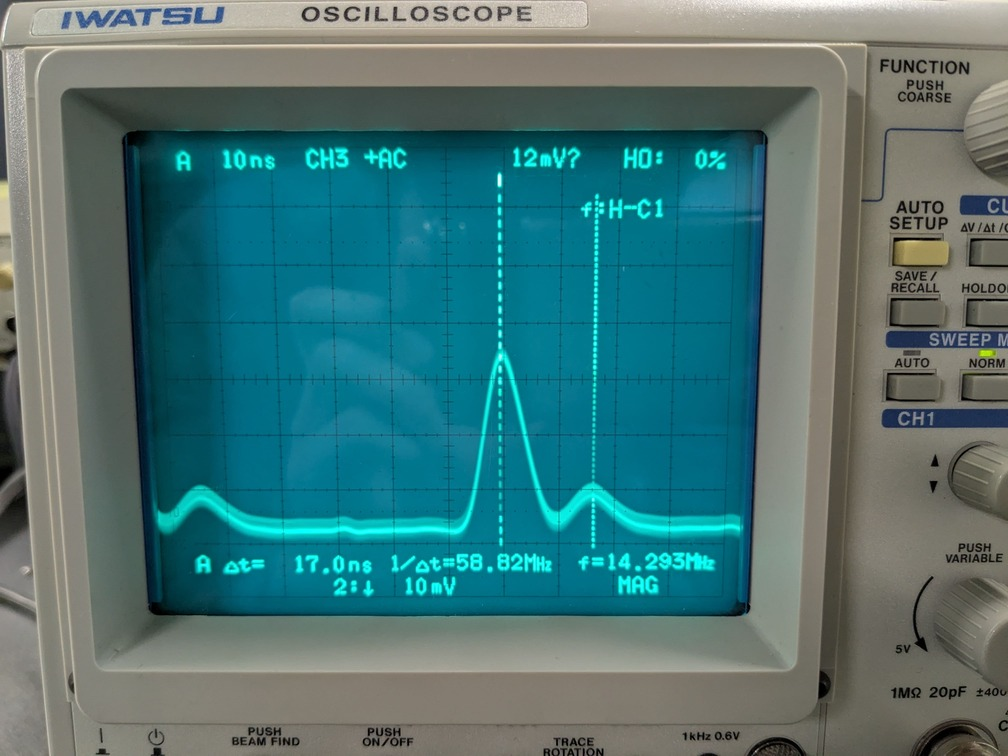
\includegraphics[scale=0.3]{lightspeed_result_picture.jpg}
    \caption{光速度計測のオシロスコープの画面}
  \end{center}
\end{figure}

\begin{table}[h]
  \centering
  \caption{光路の測定結果}
  \begin{tabular}{cccccc}
    \hline
    回数 & $d_1/\mathrm{mm}$ & $d_2/\mathrm{mm}$ & $d_3/\mathrm{mm}$ & $l_0/\mathrm{mm}$ & $l_1/\mathrm{mm}$ \\
    \hline
    1 & 2380.0 & 2864.5 & 520.5 & 177.2 & 128.2 \\
    2 & 2381.5 & 2873.0 & 522.5 & 178.1 & 128.6 \\
    3 & 2376.2 & 2872.1 & 521.2 & 178.8 & 128.8 \\
    \hline
    平均 & 2379.2 & 2869.9 & 521.4 & 178.0 & 128.5 \\
    \hline
  \end{tabular}
\end{table}

この光路の測定結果より, 光路差$L$は式(\ref{eq:L})より求められる.
[参考文献]より, プリズムのガラスの屈折率を$n=1.513$として計算すると$L=4931.1\,\mathrm{mm}$と求められる.

よって光路差$T$とパルスの時間間隔$T$より, 光速度$c$は以下のようになる.

\begin{table}[h]
  \centering
  \caption{光速度$c$の結果}
  \begin{tabular}{ccccc}
    \hline
    $L/\mathrm{mm}$ & $T/\mathrm{ns}$ & $c/\mathrm{ms^{-1}}$ & 文献値[a] & 誤差 \\
    \hline
    4931.1 & 17.0 & $2.901\times10^8$ & $2.998\times10^8$ & $0.097\times10^8$ \\
    \hline
  \end{tabular}
\end{table}


\subsection{同軸ケーブルを伝わる信号速度の測定}

以下に今回の実験で観測したオシロスコープの画面および同軸ケーブルの長さを示す.

\begin{figure}[H]
  \centering
  \begin{minipage}[b]{0.49\columnwidth}
    \centering
    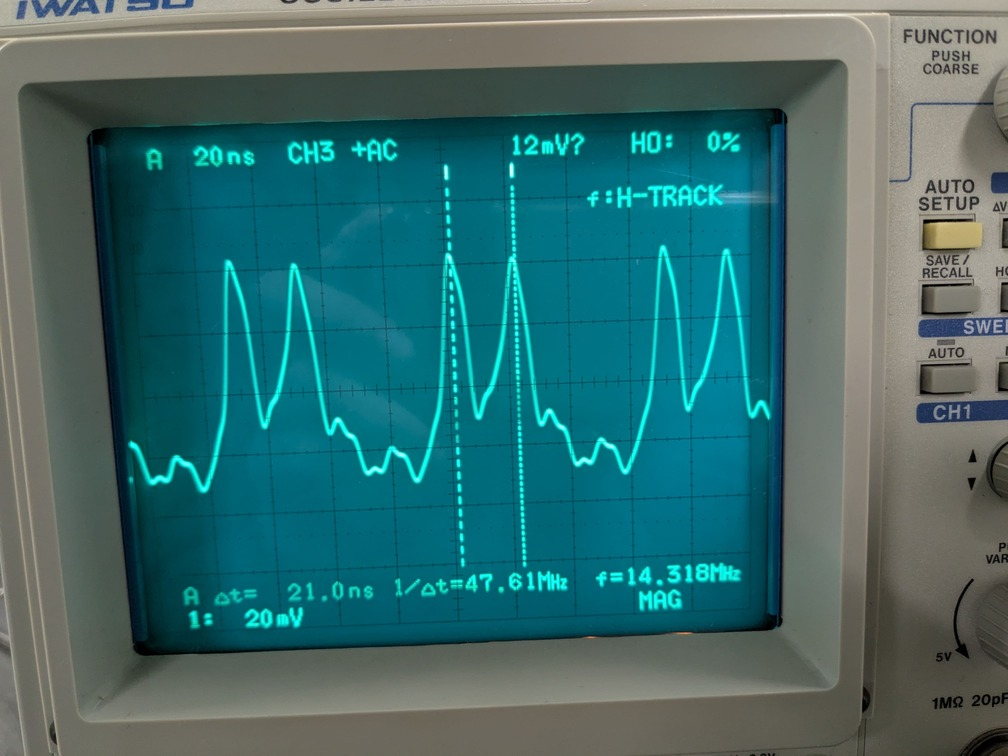
\includegraphics[scale=0.15]{cable1_result_picture.jpg}
    \caption{$L=2.04\,\mathrm{m}$}
  \end{minipage}
  \begin{minipage}[b]{0.49\columnwidth}
    \centering
    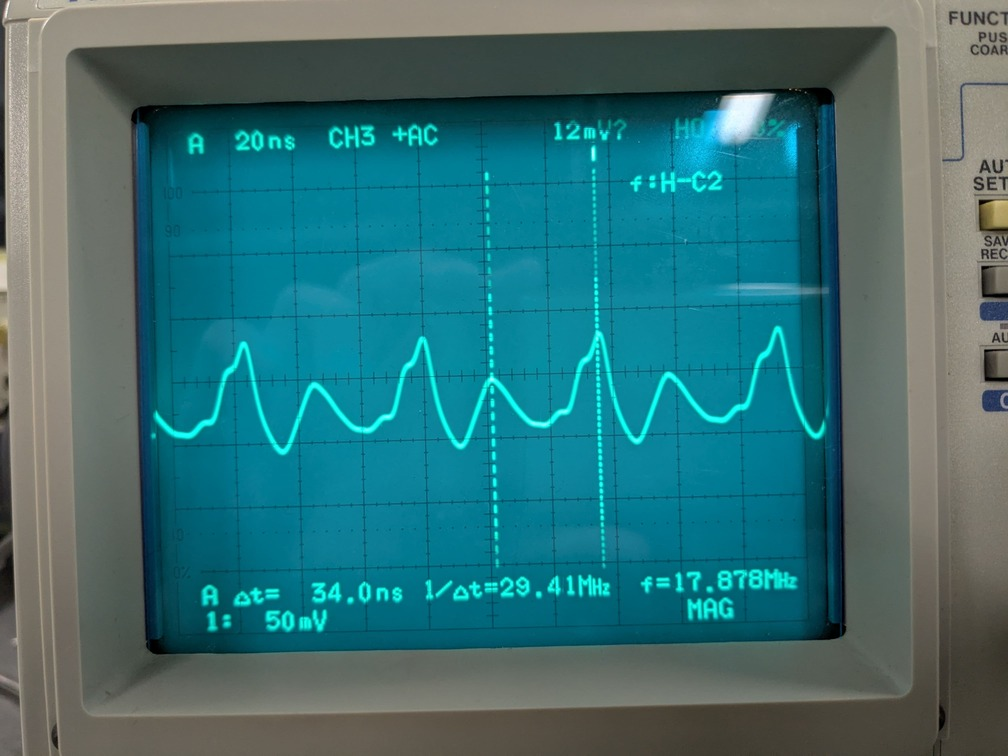
\includegraphics[scale=0.15]{cable2_result_picture.jpg}
    \caption{$L=7.61\,\mathrm{m}$}
  \end{minipage}
\end{figure}

\begin{figure}[H]
  \centering
  \begin{minipage}[b]{0.49\columnwidth}
    \centering
    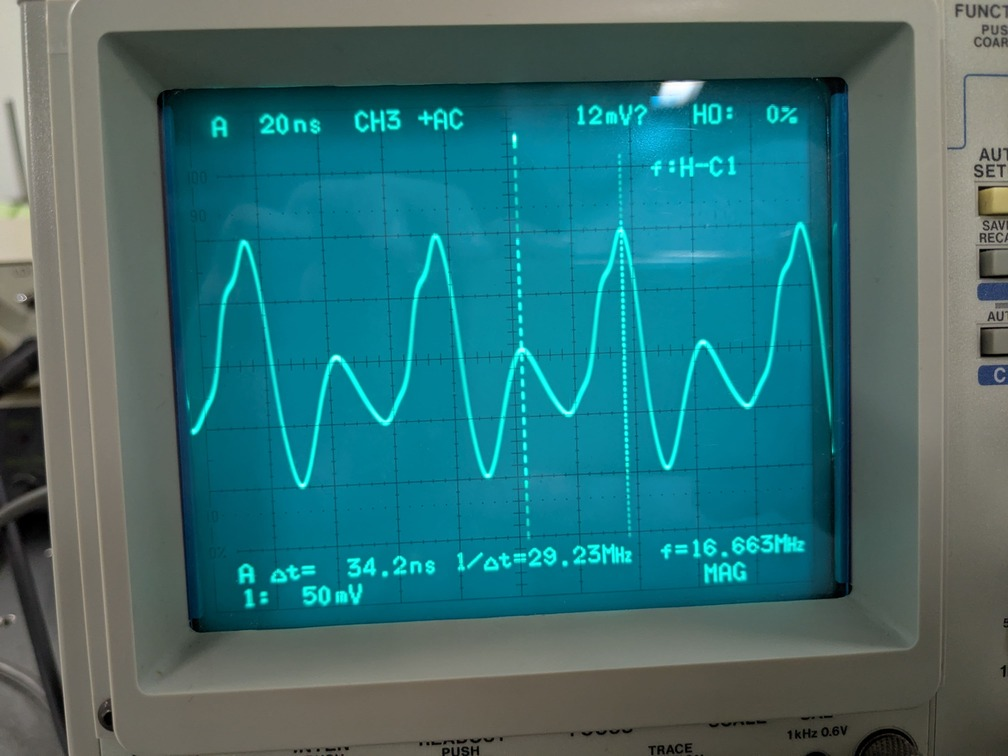
\includegraphics[scale=0.15]{cable3_result_picture.jpg}
    \caption{$L=5.06\,\mathrm{m}$}
  \end{minipage}
  \begin{minipage}[b]{0.49\columnwidth}
    \centering
    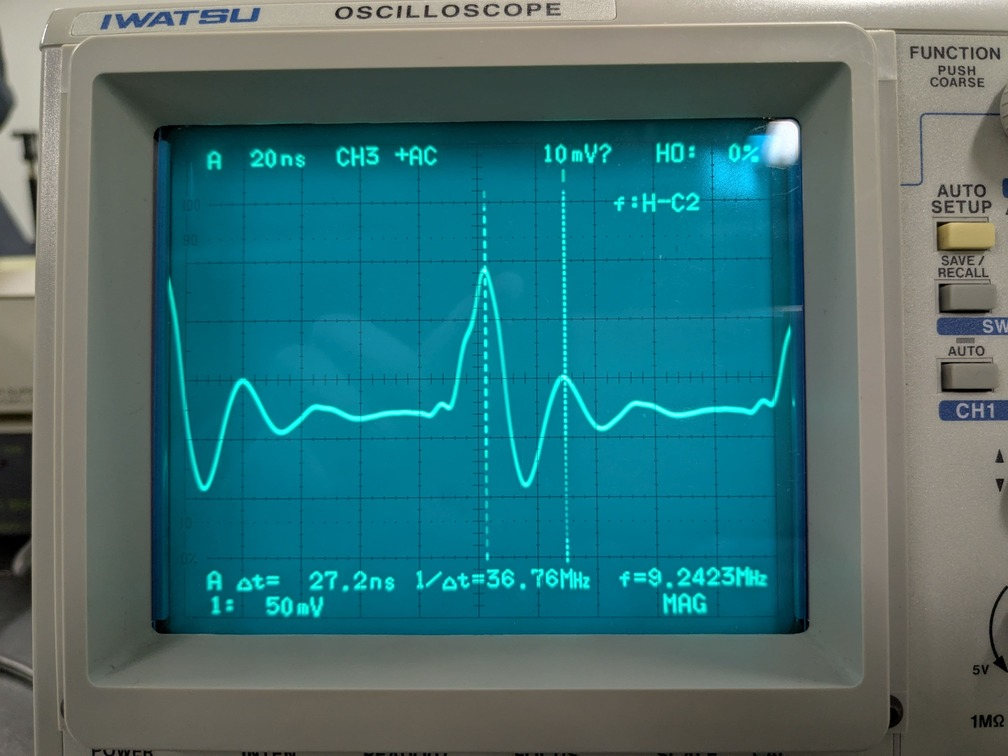
\includegraphics[scale=0.15]{cable4_result_picture.jpg}
    \caption{$L=10.03\,\mathrm{m}$}
  \end{minipage}
\end{figure}

\begin{table}[h]
  \centering
  \caption{同軸ケーブルを伝わる信号速度の測定結果}
  \begin{tabular}{ccccc}
    \hline
    ケーブル & $L/\mathrm{m}$ & $T/\mathrm{ns}$ & $v/\mathrm{ms^{-1}}$ \\
    \hline
    1 & 2.04 & 21.0 & $1.94\times10^8$ \\
    2 & 7.61 & 34.0 & $0.448\times10^8$ \\
    2 & 5.06 & 34.2 & $2.96\times10^8$ \\
    4 & 10.03 & 27.2 & $0.738\times10^8$ \\
    \hline
  \end{tabular}
\end{table}



\section{考察}


大気圧, 室温における空気の屈折率は$n=1.00028$であるが, これが今回の実験で測定した空気中の光速度について, "空気中"であって"真空中"ではないことを問題とすべきか考察する.



\begin{thebibliography}{99}


\end{thebibliography}


\end{document}